\section{State estimation}\label{sec:RealizationStateEstimation}
The rigod body controller requires the current rigid body state (position, velocity, attiude and angular velocity) and the assumed offset force and torque.
The subject of this section is the estimation of these values based on the available measurements from IMU and motion capturing system.

\paragraph{Rigid body dynamics.}
The rigid body attitude may be parameterized by a unit quaternion $\quat = [\quatw, \quatx, \quaty, \quatz] \in \Sphere^3$ which allows for a more efficient implementation of the microcontroller and is pretty common in this field.
The corresponding kinematics may be derived as proposed in \autoref{sec:MathCoordinates}.
Furthermore, using the velocity coefficients $\rd$ w.r.t. the reference frame, the rigid body dynamics are
\begin{subequations}\label{eq:RealizationStateDyn}
\begin{align}
 m (\rdd - \gravityAcc) + d \rd = \RotMatQuat(\quat) (\F + \FB)
\\
 \quatd = \kinMatQuat(\quat) \, \w, \qquad
 \bodyMOI{}{} \dot{\w} + \wedOp(\w) \bodyMOI{}{} \w = \bodyTorque{}{} + \tauB
\end{align}
with
\begin{align}
 \RotMatQuat(\quat) &=
 \begin{bmatrix} 
  1 - 2(\quaty^{2} + \quatz^{2}) & 2(\quaty\quatx -\quatw\quatz)  & 2(\quatz\quatx + \quatw\quaty) \\
  2(\quaty\quatx + \quatw\quatz) & 1 - 2(\quatx^{2} + \quatz^{2}) & 2(\quaty\quatz - \quatw\quatx) \\
  2(\quatz\quatx - \quatw\quaty) & 2(\quaty\quatz + \quatw\quatx) & 1 - 2(\quatx^{2} + \quaty^{2})
 \end{bmatrix}
\\
 \kinMatQuat(\quat) &=
 \tfrac{1}{2} \begin{bmatrix}
  -\quatx & -\quaty & -\quatz \\
  \quatw & -\quatz &  \quaty \\
  \quatz &  \quatw & -\quatx \\
  -\quaty &  \quatx &  \quatw
 \end{bmatrix}
\end{align}
\end{subequations}

\paragraph{IMU measurements.}
The \textsc{VectorNav VN100s} contains a 3-axis accelerometer, gyroscope and magnetometer connected to microcontroller which implements an extended Kalman-filter to estimate the attitude quaternion and gyroscope biases.
While the attitude estimate is used for outdoor applications with the multicopter, it is not used here, as in the lab the more precise estimate from the motion capturing system available.
%Nevertheless, we will use the bias compensated gyroscope measurement.

Gyroscope and accelerometer measure the \textit{inertial} angular velocity and acceleration.
While for tactical and navigation grade IMUs the angular velocity of the Earth is an integral part of the navigation algorithms, see e.g.\ \cite{Savage:Strapdown1}, for the consumer grade IMU here, it cannot be distinguished from the reminescent bias in gyroscope.
Similarly, the coriolis acceleration on the accelerometer may be ignored and the only external parameter is Earth's gravity $\gravityAcc$ at the current position.

The IMU is mounted to the corresponding multicopter to roughly align with its body fixed frame, more precicly the body fixed frame determined by the reflective markers for the motion capture.
We will call the remaining, constant misalgnment $\RIMUBR \in \SpecialOrthogonalGroup(3)$.
While the gyroscope bias is compensated, the accelerometer contains a noticable slowly varying bias $\aIMUB \in \RealNum^3$.
Furthermore, both sensors contain a noticable noise $\wIMUN[k], \aIMUN[k] \in \RealNum^3$ which is not further investigated here.
Overall, with a constant sampling time $\Ts=0.005\,\unit{s}$, we assume the IMU measurments $\wIMU$ and $\aIMU$ to be related to the rigid body state by:
\begin{align}
 \wIMU[k] &= \RIMUBR \w(k\Ts) + \wIMUN[k],
\\
 \aIMU[k] &=  \RIMUBR \R^\top(k\Ts) (\rdd(k\Ts) - \gravityAcc) + \aIMUB + \aIMUN[k]
 .
\end{align}

\paragraph{VICON measurements.}
The \textsc{VICON} motion capturing system measures the position $\r$ and the attitude, reported as quaternion $\quat$, by means of tracking the reflective markers on the multicopters.
The refernce frame of the system was carefully adjusted to align with gravity using a pendulum with reflective markers.

In contrast to the IMU measurments, there is no evidence for systematic errors in the measurements for the VICON system.
However, their processing and transmission to to the multicopter processor results in a substantial latency, i.e.\ measurements corresponding to time $t$ are available to the controller only after time $t+\TVICD$.
Furthermore, as non-realtime systems are involved, the latency varies slightly.
Mostly due to bandwidth limitations on the wireless transmission, the sampling time is only $\TsVIC=0.1\,\unit{s}$ while the main controller runs at $\Ts=0.005\,\unit{s}$.
The measurements $\rVIC$ and $\qVIC$ are related to the rigid body state by
\begin{align}
 \rVIC[k'] = \r(k'\TsVIC - \TVICD),
\qquad
 \qVIC[k'] = \quat(k'\TsVIC - \TVICD).
\end{align}

\begin{figure}
 \centering
 \input{graphics/StateEstimationBlock.pdf_tex}
 \caption{Overall structure of the state estimation}
 \label{fig:StateEstimationBlock}
\end{figure}

\paragraph{Overall observer design.}
Instead of designing one large observer, the estimation problem is split into smaller subproblems as illustrated in \autoref{fig:StateEstimationBlock}.
The the following subsections will discuss these.




\subsection{IMU misalignment correction}
For a static $\sysCoord=\const$ multicopter the accelerometer model is
\begin{align}
 \aIMU[k] &=  -\RIMUBR \R^\top \gravityAcc + \aIMUB + \aIMUN[k].
\end{align} 
Here we are interested in the value $\RIMUBR$, but for its estimation propsed here we also need to estimate the accelerometer bias $\aIMUN$.
For a shorttime measurment ($\Delta t<10\,\unit{min}$) is can be assumed to be constant.
Taking into account that the reference frame was carefully aligned, and the official gravitation value for Saarland, we have $\gravityAcc = [0, 0, -9.8107]^\top \tfrac{\unit{m}}{\unit{s}^2}$.

The multicopter is placed in different random orientations while the accelerometer measurements $\aIMU$ and the attitude $\R$ is recorded.
To compensate the noise $\aIMUN[k]$ we take the mean value $\bar{\tuple{a}}_{\idxText{M}}$ over $10\,\unit{s}$.
For each measurement with index $i$ and different attitudes $\bar{\R}[i]$ we have the mean accelerometer measurement $\bar{\tuple{a}}_{\idxText{M}}[i]$.
With this, we estimate the values for misalignment $\RIMUBR$ and bias $\aIMUB$ as the ones that minimize the sum over the squared errors of the experiments:
\begin{align}
 \mathcal{J}(\RIMUBR, \aIMUB) = \tfrac{1}{2} \sum_i \norm{ \bar{\tuple{a}}_{\idxText{M}}[i] + \RIMUBR \bar{\R}^\top[i] \gravityAcc + \aIMUB }^2
\end{align}
Note that this minimization problem is mathematically identical to the one considered in \autoref{sec:RBStiffness}.

\begin{figure}[htb]
 \centering
 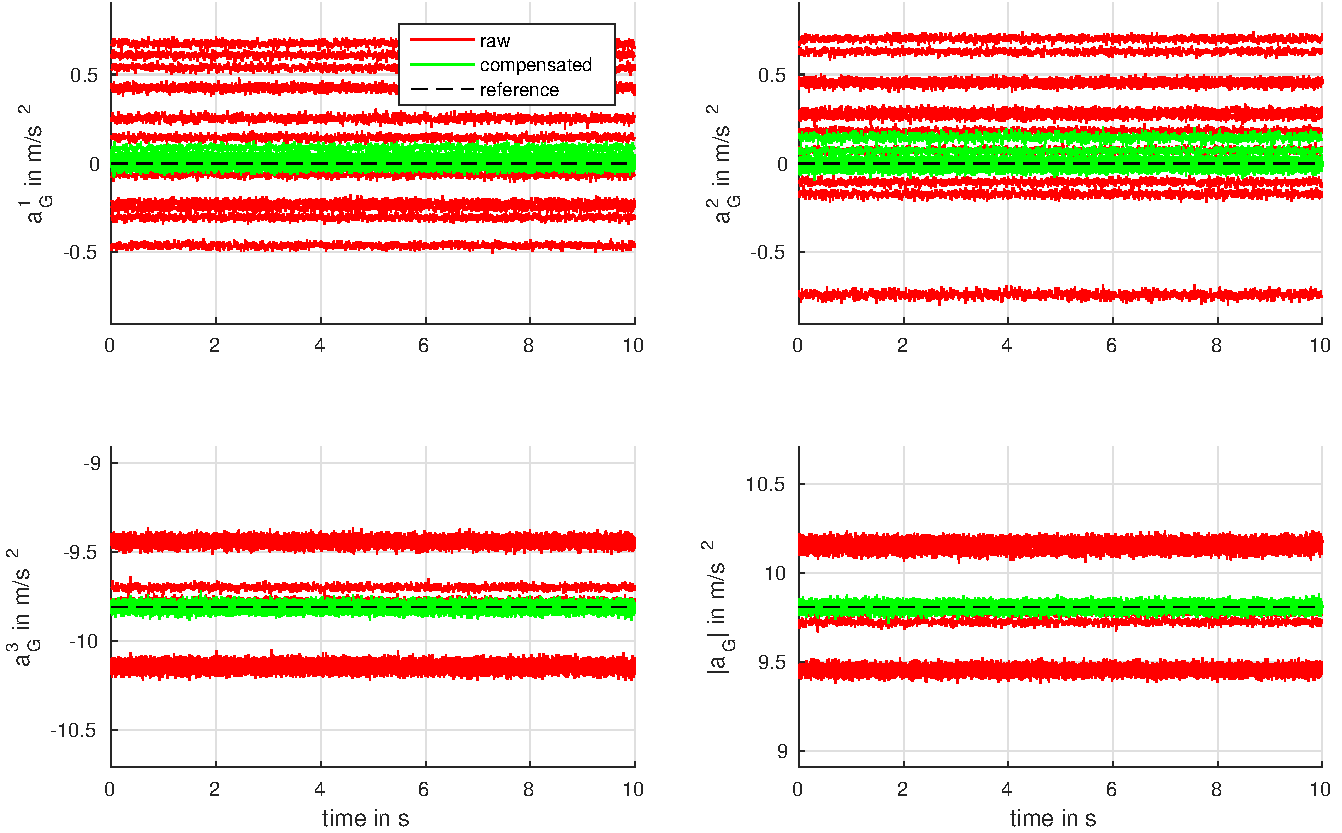
\includegraphics[scale=0.7]{AccBias.pdf}
 \caption{Accelerometer measurements and identification result}
 \label{fig:AccBias}
\end{figure}

For validation \autoref{fig:AccBias} displays the measured gravity coefficients $\gravityAcc$ within the 20 experiments with different orientations.
The red lines are the raw measurements $\gravityAcc = \RVIC \aIMU$, the green lines incorporate the identified values $\gravityAcc = \RVIC \RIMUBR (\aIMU + \aIMUB)$ and the black line is the reference value $\gravityAcc = [0,0,-9.81]^\top$.
Most notably one can see that even the magnitude $\norm{\gravityAcc}$ of the raw acceleration is off by about $5\%$ for some experiments whereas the compensated values are all within a window of about $0.2\%$.

\subsection{Angular velocity and torque bias}
Recall the mechanical model of the angular velocity $\w$, disturbance torque $\tauB$ and gyroscope $\wIMU$ motivated above:
\begin{align}
 \J \dot{\w} + \wedOp(\w) \J \w = \bodyTorque{}{} + \tauB,
\qquad
 \dot{\tau}_{\textsf{B}} = \tuple{0},
\qquad
 \wIMU = \w + \wIMUN.
\end{align}
The input torque $\bodyTorque{}{}$ is known as discussed in \autoref{sec:RealizationForceVectorControl}.

The multicopters implement a simple Luenberger observer based on the forward Euler discretization and scalar gains $L_\omega, L_\tau$: 
\begin{subequations}\label{eq:AngVelObs}
\begin{align}
 \wObs[\kPlusOne] &= \wObs[k] + \Ts \J^{-1} \big( \bodyTorque{}{}[k] + \tauBObs[k] - \wedOp(\wObs[k]) \J \wObs[k] \big) + L_\omega (\wIMU[k] - \wObs[k])
\\
 \tauBObs[\kPlusOne] &= \tauBObs[k] + L_\tau (\wIMU[k] - \wObs[k])
 .
\end{align}
\end{subequations}
In practice, the gains $L_\omega = 0.2$ and $L_\tau=0.01$ did yield good results.
The disturbance observer here takes the place of the integral controller, as the rigid body controller is "just" a PD controller.

% side calculation
% \begin{align}
%  -\wedOp(\w[k]) \Theta \w[k] + \wedOp(\wObs[k]) \Theta \wObs[k]
%  &= -\wedOp(\w[k]) \Theta \w[k] + \wedOp(\w[k] - e_\w[k]) \Theta (\w[k] - e_\w[k])
% \\
%  &= \wedOp(e_\w[k]) \Theta e_\w[k] - \wedOp(\w[k]) \Theta e_\w[k] - \wedOp(e_\w[k]) \Theta \w[k]
% \\
%  &= \wedOp(e_\w[k]) \Theta e_\w[k] + \big(\wedOp(\Theta \w[k]) - \wedOp(\w[k]) \Theta \big) e_\w[k]
% \end{align}
% \begin{align}
%  e_\w[\kPlusOne] &= e_\w[k] + \Ts e_\tau[k] - L_{\w} e_\w[k] - L_{\w} \wIMUN
% \nonumber\\
%  &\qquad \Ts \big( \wedOp(e_\w[k]) \Theta e_\w[k] + \big(\wedOp(\Theta \w[k]) - \wedOp(\w[k]) \Theta \big) e_\w[k] \big)
% \\
%  e_\tau[\kPlusOne] &= e_\tau[k] - L_\tau e_\w[k] - L_\tau \wIMUN
% \end{align}
% Introducing the error quantities $e_{\w} = \w - \wObs$ and $e_\tau = \tauB - \tauBObs$ and subtracting the observer \eqref{eq:AngVelObs} from the discretized model we find the \textit{observer error dynamics}:
% \begin{multline}\label{eq:AngVelObsErrorDyn}
%  \begin{bmatrix} e_{\w}[\kPlusOne] \\ e_{\tau}[\kPlusOne] \end{bmatrix} 
%  = \begin{bmatrix} 
%   \idMat[3] - L_{\w} - S(\w[k]) & \Ts \J^{-1} \\
%   - L_{\tau} & \idMat[3]
%  \end{bmatrix}
%  \begin{bmatrix} e_{\w}[k] \\ e_{\tau}[k] \end{bmatrix}
% \\
%  +
%  \begin{bmatrix} \Ts \J^{-1} \wedOp(e_{\w}[k]) \Theta e_{\w}[k] \\ 0 \end{bmatrix} 
%  -
%  \begin{bmatrix} L_{\w} \\ L_{\tau} \end{bmatrix} 
%  \wIMUN
% \end{multline}
% where
% \begin{align}
%  S(\w[k]) = \Ts \J^{-1} \big( \wedOp(\w[k]) \Theta - \wedOp(\Theta \w[k]) \big).
% \end{align}
% Note that the term quadratic in $e_{\w}$ is negligible if assuming small errors.
% The term $S(\w[k])$ contains the time-variant part of the error dynamics.
% However, for a reasonable gain $L_{\w}$ and typical working conditions (\eg $\norm{\w} < 10\,\sfrac{\unit{rad}}{\unit{s}}$) the gain $L_{\w}$ dominates over the time-variant part and the error dynamics are asymptotically stable.
% Furthermore, for the linearization about the hover case, $\w \approx 0$, the matrix $S$ drops out completely.
% This is used to compute the gains $L_{\w} = \diag(l_{\wx}, l_{\wy}, l_{\wz})$ and $L_{\tau} = \diag(l_{\taux}, l_{\tauy}, l_{\tauz})$ corresponding to given desired closed loop poles at this expansion point.


\subsection{Configuration measurement latency}
The configuration measurement $(\rVIC, \qVIC)$ is done by a \textsc{Vicon} motion capturing system.
This measurement relies on the optical tracking of reflective markers fixed on the multicopters by infrared cameras mounted at the walls of the lab and connected to the ground station, a Windows 7 PC.
The groundstation software is written in \textsc{Matlab}.
It runs a timer at $\TsVIC = 0.1\,\unit{ms}$ which reads the measurement, validates and forwards it to the xBee radio module.
Finally, the multicopter microcontroller receives the measurements through its ratio module.
The radio module also handles other transmitions like receiving commands and sending measurements to the groundstation.

As a result of this chain of non realtime elements, the latency at which the configuration measurements are available to the multicopter is \textit{not} constant, but varies by several main sampling steps $\Ts$ in addition to its average value.
Actual timings of these measuremnts are presented in \autoref{fig:ViconDelayIllustrate} for actual measurements.
The estimation of the resulting \textit{variable time delay} $\TVICD[k']$ is the subject of this subsection.

\begin{figure}[htb]
 \centering
 \input{graphics/ViconDelayClocks.pdf_tex}
 \caption{Illustration of the measurement time at the PC and when it is available on the microcontroller (MC)}
 \label{fig:ViconDelayClocks}
\end{figure}

To get an estimate $\TVICDObs[k']$ for this delay we utilize the clocks on the ground station PC, $t'$, and the microcontroller, $t$.
The clocks are assumed to be synchronous but have an unknown offset $\TPC = t - t' = \const$ depending on when each device was powered.
\autoref{fig:ViconDelayClocks} illustrates the time $\tVICp[k']$ at which a measurement was taken and the time $\tRec[k']$ at which it is received/available on the microcontroller.
Taking a large enough sample of these times we have the relation
\begin{align}\label{eq:meanTPC}
 \text{mean} (\tRec[1,\ldots,K'] - \tVICp[1,\ldots,K']) = \TPC + \text{mean}(\TVICD[1,\ldots,K']), \quad K'\gg 1.
\end{align}
Whereas $\TPC$ changes whenever the ground station or the micocontroller restarts, the average delay $\meanTVICD = \text{mean}(\TVICD[1,\ldots,K'])$ remains constant.

\paragraph{Experimental average delay identification.}
The identification of the average delay $\meanTVICD$ is done in a dedicated experiment:
A multicopter is mounted on an incremental encoder directly connected to the multicopter main processor.
It serves as a reference for the yaw-angle and is assumed to have negligible latency.
The encoder signal and the yaw-angle from the motion capture system are recorded by the multicopter microcontroller.
The experimental data here is about $1\,\unit{min}$ long and captures about $K' = 600$ \textsc{Vicon} frames.
Now we can plot the reference encoder angle $\yaw[k]$ at the sampling points $t = k\Ts$ and the yaw angle $\yawVIC[k']$ received from the Vicon system at the shifted time $\tVICp[k'] + \text{mean}(\tRec[1,\ldots,K'] - \tVICp[1,\ldots,K'])$.
If the previous assumption \eqref{eq:meanTPC} hold theses signals should be similar up to a shift of the mean delay $\meanTVICD$.

\begin{figure}[ht]
 \centering
 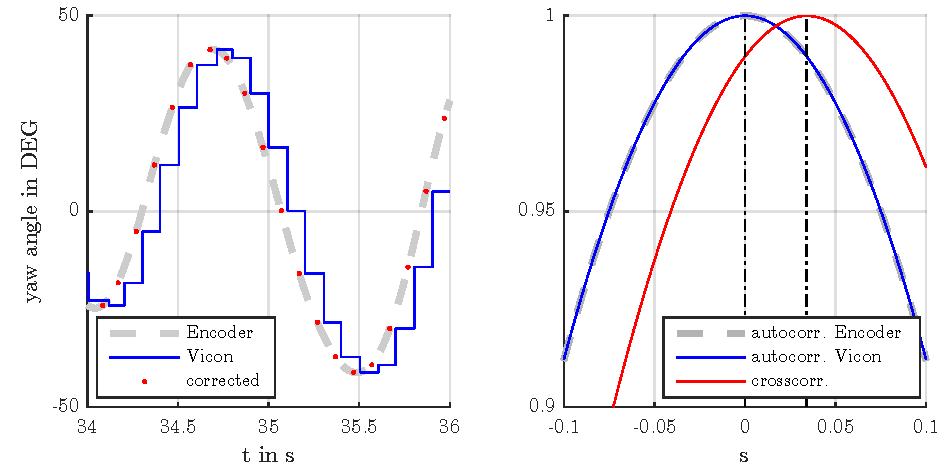
\includegraphics{ViconDelay/ViconDelayIdent.pdf}
 \caption{A small sample of the yaw-angle measurements (left) and the correlations (right) of the complete $60\,\unit{s}$ measurements for the identification of the average time delay}
 \label{fig:ViconDelayIdent}
\end{figure}

\autoref{fig:ViconDelayIdent} shows a small sample of the measured yaw angle and the correlations of the two measurements.
The identified average delay is where the cross-correlation has its maximum at $\meanTVICD = 0.034\,\unit{s}$.
In order to achieve this resolution the measurements were up-sampled to $1\,\unit{ms}$ by cubic interpolation.


\paragraph{Clock offset estimation.}
For the realtime implementation, \eqref{eq:meanTPC} is approximated by a slow ($\cTPC = 0.99$) low-pass filter
\begin{align}
 \TPCObs[k'] = \cTPC \TPCObs[k'\!-\!1] + (1-\cTPC) (\tRec[k'] - \tVICp[k'] - \meanTVICD)
\end{align}
yielding the estimate $\TPCObs$ for the constant clock offset $\TPC$.
Finally, the estimated delay of the $k'$-th Vicon measurement is
\begin{align}
 \TVICDObs[k'] = \tRec[k'] - \big( \tVICp[k'] + \TPCObs[k'] \big).
\end{align}
\autoref{fig:ViconDelayIllustrate} shows the estimated clock offset $\TPCObs$ and the resulting estimated delay $\TVICDObs$ for the previous example measurement.

\begin{figure}[ht]
 \centering
 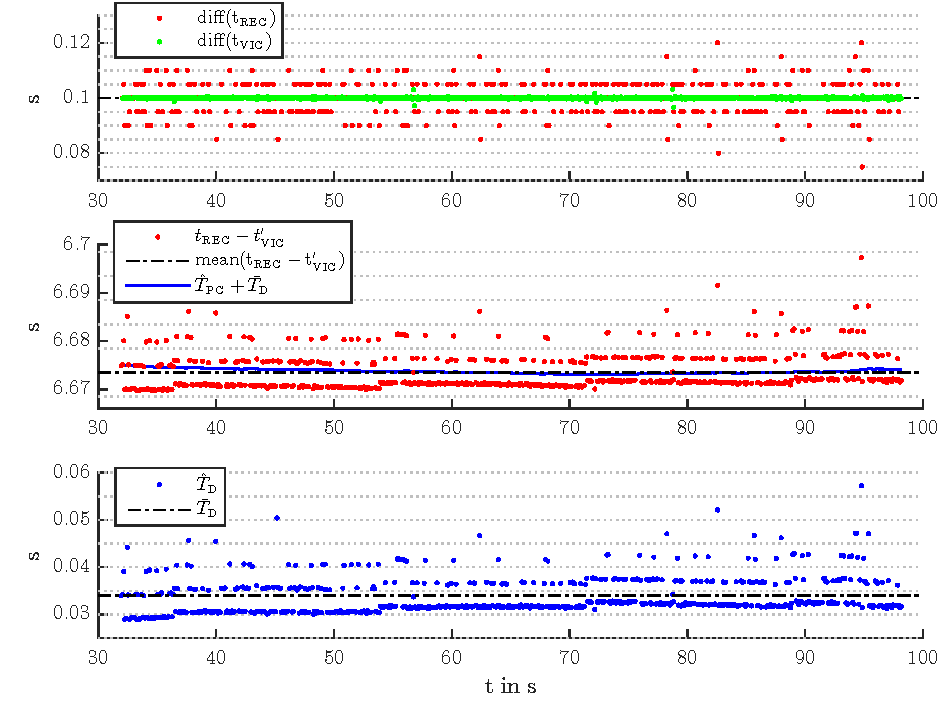
\includegraphics{graphics/ViconDelay/ViconDelayIllustrate}                                                                    
 \caption{Measured timings}
 \label{fig:ViconDelayIllustrate}
\end{figure}

\subsection{Attitude integration}
Once the latency $\TVICDObs[k']$ of the attitude measurement $\qVIC$ is known, the current attitude is simply integrated based on buffered angular velocity measurements.
The quaternion kinematics \eqref{eq:RealizationStateDyn} supplemented with a stabilization term for the constraint $\quat \in \Sphere^3$, as motivated in \autoref{sec:ConstraintStabilization}, reads
\begin{align}\label{eq:QuaternionKinematics}
 \tdiff{t} \underbrace{\begin{bmatrix} \quatw \\ \quatx \\ \quaty \\ \quatz \end{bmatrix}}_{\quat}
 = \underbrace{\tfrac{1}{2} \begin{bmatrix} -\quatx & -\quaty & -\quatz \\ \quatw & -\quatz & \quaty \\ \quatz & \quatw & -\quatx \\ -\quaty & \quatx & \quatw \end{bmatrix}}_{\kinMatQuat(\quat)}
 \underbrace{\begin{bmatrix} \wx \\ \wy \\ \wz \end{bmatrix}}_{\w}
 -
 \underbrace{\tfrac{1}{2} \begin{bmatrix} \quatw \\ \quatx \\ \quaty \\ \quatz \end{bmatrix}}_{\left(\pdiff[\geoConstraint]{\quat}(\quat)\right)^+}
 \lambda\underbrace{(\norm{\quat}^2 - 1)}_{\geoConstraint(\quat)}
 .
\end{align}
The actual implementation uses the forward Euler discretization with the stabilization gain $\lambda=\sfrac{2}{\Ts}$, i.e.\
\begin{align}\label{eq:QuaternionKinematicsDiscrete}
 \quat[k\!+\!1] = \quat[k] + \Ts \kinMatQuat(\quat[k]) \w[k] - (\norm{\quat[k]}^2-1) \quat[k].
\end{align}
Note that with this particular gain the stabilization coincides with the 1st order Taylor expansion of the normalization $\sfrac{\quat}{\norm{\quat}} \approx \quat - (\norm{\quat}^2-1) \quat$ for $\norm{\quat} \approx 1$.
In contrast to the exact normalization, the approximation avoids the expensive computation of a square root and division.

% \paragraph{Attitude integration.}
% From the previous subsection we know the micro controller time $\tVIC[k'] = \tRec[k'] - \TVICDObs[k']$ at which the received attitude measurement $\qVIC[k']$ was taken.
% To get the an estimate $\quatObs[k]$ for the current attitude we \textit{integrate} the attitude quaternion kinematics \eqref{eq:QuaternionKinematicsDiscrete} using the measurement $\qVIC[k']$ as initial value and the (ring) buffered angular velocity estimates $\wObs[k-\text{floor}(\sfrac{\TVICDObs[k']}{\Ts})],\ldots, \wObs[k]$.
% Since the delay $\TVICDObs[k']$ is usually not a multiple of the micro controller sampling time $\Ts$ a linear interpolation of the angular velocity $\wObs(\tVIC[k'])$ is used.


\subsection{Position, velocity and accelerometer bias}
For the translational dynamics we have a similar situation as for the attitude kinematics:
We have a down-sampled and delayed position measurement $\rVIC$ and a biased and noisy measurement of the acceleration $\aIMU$.
From this we want to estimate the current position $\r$ and velocity $\rd$ required for the controller implementation.

The relation between position and accelerometer measurement and the differential equation for a constant accelerometer bias are
% \begin{align}
%  \rdd = \gravityAcc + \R (\aIMU - \aIMUB - \aIMUN),
% \qquad
%  \aIMUBd = 0
% \end{align}
% A discrete approximation for this is
% \begin{multline}\label{eq:AccelerometerDynamicsDiscrete}
%  \underbrace{\begin{bmatrix} \r[\kPlusOne] \\ \rd[\kPlusOne] \\ \aIMUB[\kPlusOne] \end{bmatrix}}_{z[\kPlusOne]}
%  =
%  \underbrace{\begin{bmatrix} \idMat[3] & \Ts\idMat[3] & -\tfrac{\Ts^2}{2}\R[k] \\ 0 & \idMat[3] & -\Ts\R[k] \\ 0 & 0 & \idMat[3] \end{bmatrix}}_{A[k]}
%  \underbrace{\begin{bmatrix} \r[k] \\ \rd[k] \\ \aIMUB[k] \end{bmatrix}}_{z[k]}
%  +
%  \underbrace{\begin{bmatrix} \tfrac{\Ts^2}{2}\idMat[3] \\ \Ts \idMat[3] \\ 0 \end{bmatrix}}_{B}
%  \big(\underbrace{\gravityAcc + \R[k] \aIMU[k]}_{u[k]} - \underbrace{R[k] \aIMUN[k]}_{u_{\mathsf{N}}[k]} \big)
% % -
% % \underbrace{\begin{bmatrix} \tfrac{\Ts^2}{2}\idMat[3] \\ \Ts \idMat[3] \\ 0 \end{bmatrix} \R[k] \aIMUN[k]}_{u_{\mathsf{N}}[k]}
% \end{multline}
% Note that this approximation assumes that the attitude $\R$ is constant within one sampling step.
% If this would be the case, the discretization would be exact.
\begin{align}
 \aIMU = \R^\top(\rdd - \gravityAcc) + \aIMUB + \aIMUN,
\qquad
 \aIMUBd = 0
\end{align}
Introducing the state $z = [\r^\top, \rd^\top, \aIMUB^\top]^\top$ and neglecting the accelerometer noise $\aIMUN=0$, this can be written as
\begin{align}\label{eq:AccelerometerDynamicsState}
 \tdiff{t}
 \underbrace{\begin{bmatrix} \r \\ \rd \\ \aIMUB \end{bmatrix}}_{z}
 &=
 \underbrace{\begin{bmatrix} 0 & \idMat[3] & 0 \\ 0 & 0 & -\R \\ 0 & 0 & 0 \end{bmatrix}}_{A}
 \underbrace{\begin{bmatrix} \r \\ \rd \\ \aIMUB \end{bmatrix}}_{z}
 +
 \underbrace{\begin{bmatrix} 0 \\ \idMat[3] \\ 0 \end{bmatrix}}_{B}
 \underbrace{(\gravityAcc + \R \aIMU)}_{u}
\end{align}

\paragraph{Estimator implementation.}
The implemented estimation algorithm on the \microcontroller works as follows:
After having received 2 subsequent position measurements $\rVIC[1]$, $\rVIC[2]$ and their reconstructed time $\tVIC[1]$, $\tVIC[2]$ with $\Ts'[1]=\tVIC[2]-\tVIC[1]$ we set the initial value for the estimator state $\hat{z} = [\rObs^\top, \rdObs^\top, \aIMUBObs^\top]^\top$ as
\begin{align}
 \rObs(\tVIC[2]) = \rVIC[2], 
\qquad
 \rdObs(\tVIC[2]) = \tfrac{\rVIC[2]-\rVIC[1]}{\Ts'[1]}
\qquad
 \aIMUB(\tVIC[2]) = 0.
\end{align}
Then a discrete approximation of the accelerometer dynamics \eqref{eq:AccelerometerDynamicsState}:
\begin{align}\label{eq:PosPredictor}
 \underbrace{\begin{bmatrix} \rObs[\kPlusOne] \\ \rdObs[\kPlusOne] \\ \aIMUBObs[\kPlusOne] \end{bmatrix}}_{\hat{z}[\kPlusOne]}
 =
 \underbrace{\begin{bmatrix} \idMat[3] & \Ts\idMat[3] & -\tfrac{\Ts^2}{2}\RObs[k] \\ 0 & \idMat[3] & -\Ts\RObs[k] \\ 0 & 0 & \idMat[3] \end{bmatrix}}_{\hat{A}_\idxSamp[k]}
 \underbrace{\begin{bmatrix} \rObs[k] \\ \rdObs[k] \\ \aIMUBObs[k] \end{bmatrix}}_{\hat{z}[k]}
 +
 \underbrace{\begin{bmatrix} \tfrac{\Ts^2}{2}\idMat[3] \\ \Ts \idMat[3] \\ 0 \end{bmatrix}}_{B_\idxSamp}
 \underbrace{(\gravityAcc + \RObs[k] \aIMU[k])}_{\hat{u}[k]}
\end{align}
is used to integrate the current position and velocity.
Note that the measurement time $\tVIC[2]$ usually does not coincide with a sampling step, see \autoref{fig:ViconDelayClocks}.
Consequently the value $\Ts$ in \eqref{eq:PosPredictor} has to be adjusted to match the time from the initial value to the subsequent sampling step.
Furthermore the accelerometer measurement $\aIMU$ is linearly interpolated to approximate the acceleration at the initial time $\tVIC[2]$.
The attitude $\R$ at the initial point is $\RotMatQuat(\qVIC[2])$ which is received simultaneously with $\rVIC[2]$.

After this initial procedure, \eqref{eq:PosPredictor} is computed once every sampling step with the most recent accelerometer measurement $\aIMU[k]$ yielding the most recent predictions for the position and velocity.
The position estimates $\rObs[k]$ for the last 64 sampling steps are stored in a ring buffer.

When a new configuration measurement $(\rVIC[k'], \RVIC[k'])$ and its timestamp $\tVIC[k']$ are available, the corresponding estimate $\rObs(\tVIC[k'])$ is interpolated.
This is used to correct the estimate \textit{at the measurement time} $\tVIC[k']$, i.e.\
\begin{align}\label{eq:PosCorrector}
 \underbrace{\begin{bmatrix} \rObs(\tVIC[k']) \\ \rdObs(\tVIC[k']) \\ \aIMUBObs(\tVIC[k']) \end{bmatrix}}_{\hat{z}(\tVIC[k'])}
 \leftarrow 
 \underbrace{\begin{bmatrix} \rObs(\tVIC[k']) \\ \rdObs(\tVIC[k']) \\ \aIMUBObs(\tVIC[k']) \end{bmatrix}}_{\hat{z}(\tVIC[k'])}
 +
 \underbrace{\begin{bmatrix} L_r[k'] \\ L_v[k'] \\ L_a[k'] (\RVIC[k'])^\top \end{bmatrix}}_{L[k']}
 (\rVIC[k'] - \rObs(\tVIC[k'])).
\end{align}
After the correction the prediction for the current sampling step is again integrated from \eqref{eq:PosPredictor}.
Note that this also requires a (ring) buffer for the last accelerometer measurements.

\paragraph{Error dynamics and tuning.}
To chose reasonable correction gains $L_r$, $L_v$ and $L_a$ we investigate the resulting error dynamics of the proposed estimator.
Here we do the coarse assumption that the attitude is constant and perfectly known $\RObs = \bar{\R}$.
Then the dynamic matrix $A$ in the continuous model \eqref{eq:AccelerometerDynamicsState} is constant and is denoted by $\bar{A}$.

From measurement time $\tVIC[k']$ till the next one at $\tVIC[k'+1]$ there are several prediction steps \eqref{eq:PosPredictor}:
The first from the measurement time till the subsequent sampling step with integration time $T_\mathsf{I}$.
Then several steps with integration time $\Ts$ till the sampling step before $\tVIC[k'+1]$, and finally a step integration time $T_\mathsf{F}$ till $\tVIC[k'+1]$.
Overall this results in the dynamic matrix 
\begin{align}
 \bar{A}'_\idxSamp = \exp(\bar{A}\,T_\mathsf{I}) \exp(\bar{A}\,\Ts) \cdots \exp(\bar{A}\,\Ts) \exp(\bar{A}\,T_\mathsf{F}) = \exp(\bar{A}\,\Tsp), 
\end{align}
where $\Tsp[k'] = T_\mathsf{I}[k'] + \Ts + \ldots + \Ts + T_\mathsf{F}[k'] = \tVIC[k'] - \tVIC[k'-1]$.
Since $\Tsp[k']$ is known and exploiting this property of the exponential map, we do not need to worry about the different integration times of the predictions.

Finally we add one correction step \eqref{eq:PosCorrector} and subtract the estimator from the discretization of the model \eqref{eq:AccelerometerDynamicsState} to obtain the relation for the error $e = z - \hat{z}$ at one correction/measurement time $\tVIC[k']$ to the next one at $\tVIC[k'+1]$ as
\begin{align}
 e(\tVIC[k'\!+\!1]) = \underbrace{(\idMat[9] - \bar{L}[k'] C) \bar{A}'_\idxSamp[k']}_{\bar{A}'_e[k']} e(\tVIC[k'])
\end{align}
where
\begin{align}
 \bar{A}'_\idxSamp[k'] &=
 \begin{bmatrix}
  \idMat[3] & \Tsp[k'] \idMat[3] & -\tfrac{(\Tsp[k'])^2}{2} \bar{\R} \\
  0 & \idMat[3] & -\Tsp[k']\bar{\R} \\
  0 & 0 & \idMat[3]
 \end{bmatrix},&
 \bar{L}[k'] &= \begin{bmatrix} L_r[k'] \\ L_v[k'] \\ L_a[k'] \bar{\R}^\top \end{bmatrix},&
 C &= [\idMat[3] \ 0 \ 0]
\end{align}
and finally
\begin{align}
 \bar{A}_e[k'] = 
 \begin{bmatrix} 
  \idMat[3] - L_r[k'] & \Tsp(\idMat[3] - L_r[k']) & \tfrac{(\Tsp[k'])^2}{2}(L_r[k'] - \idMat[3]) \bar{\R} \\
  -L_v[k'] & \idMat[3] - \Tsp[k'] L_v[k'] & \Ts(\tfrac{\Tsp[k']}{2} L_v[k'] - \idMat[3])\bar{\R} \\
  -L_a[k'] \bar{\R}^\top & -\Tsp[k'] L_a[k'] \bar{\R}^\top & \idMat[3] + \tfrac{\Tsp[k']^2}{2} L_a[k']
 \end{bmatrix}
%  \begin{bmatrix} 
%   (1-l_r)\idMat[3] & \Ts'(1 - l_r)\idMat[3] & \tfrac{\Ts'^2}{2}(l_r - 1) \bar{\R} \\
%   -l_v \idMat[3] & (1-\Ts'l_v)\idMat[3] & \Ts(\tfrac{\Ts'}{2}l_v - 1) \bar{\R} \\
%   -l_a \bar{\R}^\top & -\Ts' l_a \bar{R}^\top & (1 + \tfrac{\Ts'^2}{2} l_a) \idMat[3]
%  \end{bmatrix}
\end{align}
Scaling the gains with the variable integration time $\Tsp[k']$ between two correction steps as
\begin{align}
 L_r[k'] &= l_r \idMat[3],& 
 L_v[k'] &= \tfrac{l_v}{\Tsp[k']} \idMat[3],&
 L_a[k'] &= \tfrac{2 l_a}{(\Tsp[k'])^2}
\end{align}
yields the characteristic polynomial with constant coefficients
\begin{align}
 \det(\lambda \idMat[9] - \bar{A}'_e[k'])
 = \Big( \lambda^3
  + \big(l_r + l'_v - l'_a - 3 \big) \lambda^2
  + \big(3 - 2 l_r - l'_v - l'_a \big) \lambda
  + l_r - 1
 \Big)^3.
\end{align}
However, it should be noted here that constant eigenvalues of the time varying matrix $\bar{A}'_e[k']$ can not conclude stability of the time-varying system.

In practice the eigenvalues $\eig(\bar{A}'_e) = \{ 0, 0.5, 0.9 \}$ and the resulting gains $l_r = 1$, $l_v = 0.575$, $l_a = -0.025$ did result in quite good estimation performance.
These rather fast eigenvalues also reflect a high confidence in the position measurement.


\subsection{Force bias}
Recall the translational \Multicopter dynamics and the accelerometer measurement $\aIMU$ equation
\begin{align}
 m (\rdd - \gravityAcc) + d \rd &= \R (F + \FB),&
 \aIMU &= \RT (\ddot{r} - \gravityAcc) + \aIMUN + \aIMUB.
\end{align}
Solving these equations for the force bias $\FB$ and elimination of the acceleration $\rdd$ yields
\begin{align}
 \FB &= m (\aIMU - \aIMUN - \aIMUB) + d \RT \dot{r} - F.
\end{align}
From the previous subsections we have estimates for the attitude $\RObs$, velocity $\rdObs$ and the accelerometer bias $\aIMUBObs$.
From the previous section on the actuator dynamics we have a an estimate for the \Multicopter force $\FObs$.
However, the accelerometer measurement $\aIMU$ contains the significant, unknown noise $\aIMUN$.
In order to suppress this noise we use a simple low-pass to obtain the estimate $\FBObs$ for the force bias
\begin{align}
 \FBObs[\kPlusOne] = l_F \FBObs[k] + (1 - l_F) \big( m (\aIMU[k] - \aIMUBObs[k]) + d (\RObs[k])^\top \rdObs[k] - \FObs[k] \big)
 .
\end{align}
In practice the low-pass gain $l_F = 0.98$ did yield reasonable results.
